%%%%%%%%%%%%%%%%%%%%%%%%%%%%%%%%%%%%%%%%%%%%%%%%%%%%%%%%%%%%%%%%%%%%%%%%%%%%%%%%
%%%%%%%%%%%%%%%%%%   Vorlage für eine Abschlussarbeit   %%%%%%%%%%%%%%%%%%%%%%%%
%%%%%%%%%%%%%%%%%%%%%%%%%%%%%%%%%%%%%%%%%%%%%%%%%%%%%%%%%%%%%%%%%%%%%%%%%%%%%%%%

% Erstellt von Maximilian Nöthe, <maximilian.noethe@tu-dortmund.de>
% ausgelegt für lualatex und Biblatex mit biber

% Kompilieren mit
% latexmk --lualatex --output-directory=build thesis.tex
% oder einfach mit:
% make

\documentclass[
  tucolor,       % remove for less green,
  BCOR=12mm,     % 12mm binding corrections, adjust to fit your binding
  parskip=half,  % new paragraphs start with half line vertical space
  open=any,      % chapters start on both odd and even pages
  cleardoublepage=plain,  % no header/footer on blank pages
]{tudothesis}


% Warning, if another latex run is needed
\usepackage[aux]{rerunfilecheck}

% just list chapters and sections in the toc, not subsections or smaller
\setcounter{tocdepth}{1}

%------------------------------------------------------------------------------
%------------------------------ Fonts, Unicode, Language ----------------------
%------------------------------------------------------------------------------
\usepackage{fontspec}
\defaultfontfeatures{Ligatures=TeX}  % -- becomes en-dash etc.

% load english (for abstract) and ngerman language
% the main language has to come last
\usepackage[american, british]{babel}

% intelligent quotation marks, language and nesting sensitive
\usepackage[autostyle]{csquotes}

% microtypographical features, makes the text look nicer on the small scale
\usepackage{microtype}

%------------------------------------------------------------------------------
%------------------------ Math Packages and settings --------------------------
%------------------------------------------------------------------------------

\usepackage{amsmath}
\usepackage{amssymb}
\usepackage{mathtools}

% Enable Unicode-Math and follow the ISO-Standards for typesetting math
\usepackage[
  math-style=ISO,
  bold-style=ISO,
  sans-style=italic,
  nabla=upright,
  partial=upright,
  warnings-off={mathtools-colon,mathtools-overbracket}, % suppress some unnecessary warnings
]{unicode-math}
\setmathfont{Latin Modern Math}

% nice, small fracs for the text with \sfrac{}{}
\usepackage{xfrac}


%------------------------------------------------------------------------------
%---------------------------- Numbers and Units -------------------------------
%------------------------------------------------------------------------------

\usepackage[
  locale=DE,
  separate-uncertainty=true,
  per-mode=symbol-or-fraction,
]{siunitx}

%------------------------------------------------------------------------------
%-------------------------------- tables  -------------------------------------
%------------------------------------------------------------------------------

\usepackage{booktabs}       % \toprule, \midrule, \bottomrule, etc

%------------------------------------------------------------------------------
%-------------------------------- graphics -------------------------------------
%------------------------------------------------------------------------------

\usepackage{graphicx}
\usepackage{wrapfig}
% currently broken
% \usepackage{grffile}

% allow figures to be placed in the running text by default:
\usepackage{scrhack}
\usepackage{float}
\floatplacement{figure}{htbp}
\floatplacement{table}{htbp}

% keep figures and tables in the section
\usepackage[section, below]{placeins}

% allows to include PDFs as full pages
\usepackage{pdfpages}

% Set the PDF Version of this document to 1.7 (1.4 is the current default)
% This is needed so that PDFs with Version >1.5 can be included
\pdfvariable minorversion=7

%------------------------------------------------------------------------------
%---------------------- customize list environments ---------------------------
%------------------------------------------------------------------------------

\usepackage{enumitem}

%------------------------------------------------------------------------------
%------------------------------ Bibliographie ---------------------------------
%------------------------------------------------------------------------------

\usepackage[
  backend=biber,   % use modern biber backend
  autolang=hyphen, % load hyphenation rules for if language of bibentry is not
                   % german, has to be loaded with \setotherlanguages
                   % in the references.bib use langid={en} for english sources
  sorting=none,   % sort bibliography by appearance
]{biblatex}
\addbibresource{references.bib}  % the bib file to use
\DefineBibliographyStrings{german}{andothers = {{et\,al\adddot}}}  % replace u.a. with et al.
% \bibliographystyle{unsrt}


% Last packages, do not change order or insert new packages after these ones
\usepackage[pdfusetitle, unicode, linkbordercolor=tugreen, citebordercolor=tugreen]{hyperref}
\usepackage{bookmark}
\usepackage[shortcuts]{extdash}

%------------------------------------------------------------------------------
%-------------------------    Angaben zur Arbeit   ----------------------------
%------------------------------------------------------------------------------

\author{Joel Koch}
\title{Detecting Brain Tumours using a Convolutional Neural Network}
\subtitle{Seminar: Machine Learning for Physicists}
\date{31.07.2024}
% \birthplace{Castrop-Rauxel}
\chair{Experimental Physics IV}
\division{Faculty Physics}

% tu logo on top of the titlepage
\titlehead{\includegraphics[height=1.5cm]{../logo_engl.pdf}}

\begin{document}
\frontmatter
\maketitle

% Gutachterseite
% \makecorrectorpage

% hier beginnt der Vorspann, nummeriert in römischen Zahlen
% \thispagestyle{plain}

\section*{Kurzfassung}
Hier steht eine Kurzfassung der Arbeit in deutscher Sprache inklusive der Zusammenfassung der
Ergebnisse.
Zusammen mit der englischen Zusammenfassung muss sie auf diese Seite passen.

\section*{Abstract}
\begin{foreignlanguage}{english}
The abstract is a short summary of the thesis in English, together with the German summary it has to fit on this page.
\end{foreignlanguage}

\tableofcontents

\mainmatter
% Hier beginnt der Inhalt mit Seite 1 in arabischen Ziffern
\chapter{Introduction}
\label{cha:introduction}

To detect brain tumours and classify them into malignant and benign, is a vital challenge in the field of medical diagnostics. 
Accurate and timely diagnosis is essential for effective treatment planning and improving the patient's health.
Traditional methods for diagnosing brain tumours are biopsies or manually evaluating medical images like magnetic resonance imaging (MRI) scans \cite{CancerResearUK}.
These methods are time-consuming, expensive, and can be error-prone. 
With advancements in the field of machine learning, it is possible to automate the process of diagnosing brain tumours using machine learning techniques. %convolutional neural networks (CNNs).
To use machine learning, the brain tumour which is to be classified as malignant or benign, needs to be analysed by a doctor into certain features.
These features can be extracted from MRI scans and used as input for a machine-learning model.
To overcome this analysis step, a neural network can be trained on the MRI scans themselves.
A task such as this is known as image classification.
Convolutional neural networks (CNNs) are a type of artificial neural network that is well-suited for image classification tasks, by applying filters to input images to detect patterns.

A CNN to classify brain tumours in MRI scans as malignant or benign is developed in this work.
This model is compared to binary classification models to evaluate its performance, such as logistic regression, support vector machines, and k-nearest neighbours.
The metric used to evaluate the models is the recall score, as it is important to detect malignant tumours correctly.

The dataset used in this work is the "Brain Tumor" dataset from Kaggle \cite{jakesh_bohaju_2020}.
It contains 3762 images with labels that can be used for the CNN.
It also contains five first-order and eight second-order features that can be used for the binary classification methods and described later.
% The first-order features are mean, variance, skewness, kurtosis, and entropy.
% The second-order features are contrast, energy, angular second moment (ASM), entropy, homogeneity, dissimilarity, correlation, and coarseness.
The dataset runs under the Creative Commons license, which allows for sharing and adapting the dataset for non-commercial purposes \href{https://creativecommons.org/licenses/by-nc-sa/4.0/}{(CC BY-NC-SA 4.0)}. 
% The CNN is trained on the images from the dataset, and the binary classification models are trained on the features extracted from the images.

The CNN is explained in more detail in chapter \ref{cha:CNN}, where the network architecture, the initial model, the hyperparameter optimization, and the final model are discussed.
The binary classification models are explained in chapter \ref{cha:alternative_methods} and a comparison between the CNN and the binary classification models is made in section \ref{sec:comparison}.
% A comparison between the CNN and the binary classification models is made in section \ref{sec:comparison}.
A discussion and an outlook are given in chapter \ref{cha:conclusion}. 
The code can be found in the corresponding GitHub repository \cite{project} or directly via the \href{https://github.com/joeyko2706/MachineLearning24/tree/main}{link}.

% \section{Dataset}
% \label{sec:dataset}



% \cite{tensorflow}
% \begin{figure}[H]
%     \centering
%     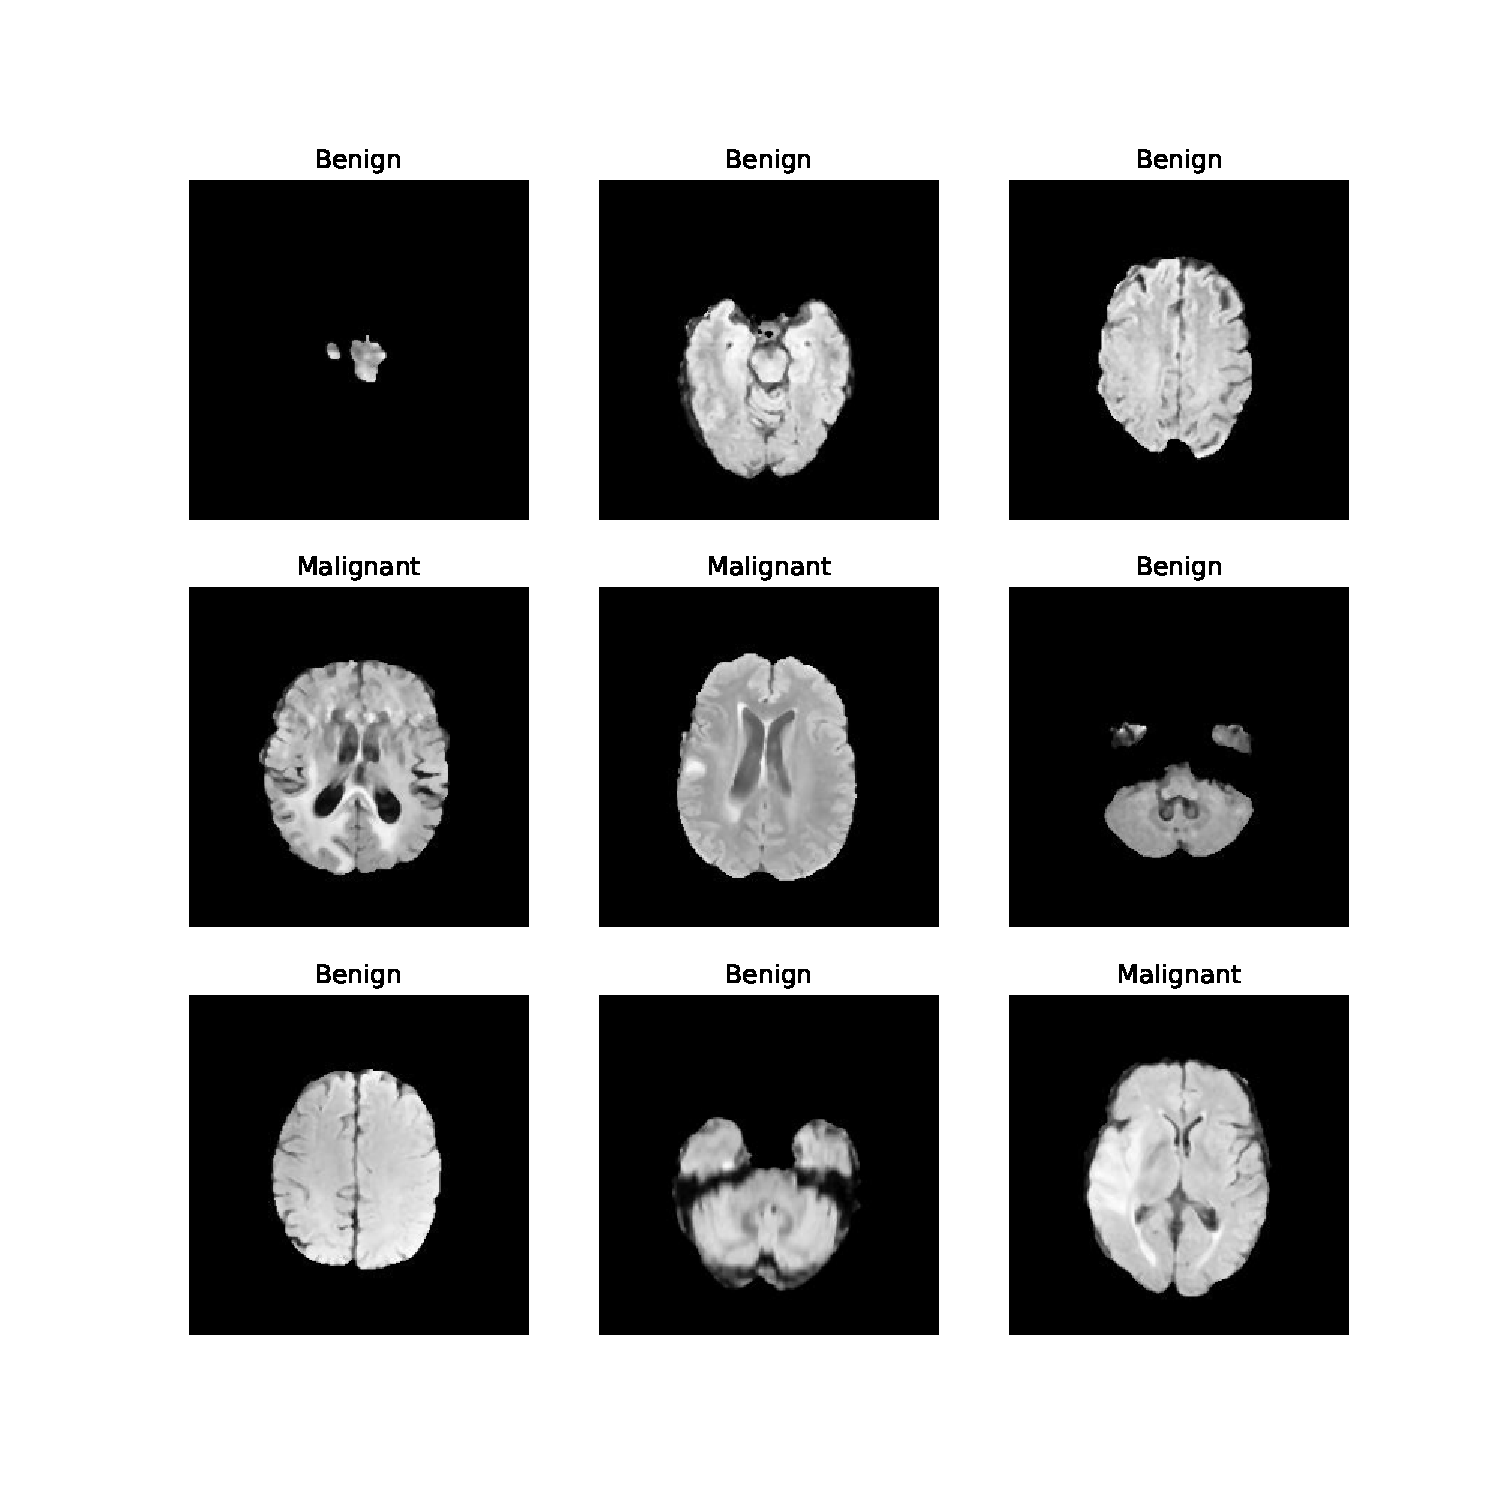
\includegraphics[width=.8\textwidth]{plots/tumor_images.pdf}
%     \caption{Malignant and benign tumour images from the dataset.}
%     \label{fig:tumorImages}
% \end{figure}

\chapter{Convolutional Neural Network}
\label{cha:CNN}

The dataset consists of two classes, the training and the test dataset. 
The training dataset is split into a training and a validation subset, containing 80\% and 20\% of the data, leading to 2408 and 602 samples, respectively.
The test dataset contains 752 samples.
The images are grayscale and have a size of $240 \times 240$ pixels.
As it is much more dangerous for a patient to have a malignant tumour classified as benign than the other way around, recall is used as the main metric to evaluate the models.
During the training, however, the model is optimized using the accuracy.
% The recall is defined as the ratio of the true positive predictions to the sum of the true positive and false negative predictions.
Benign tumours are labelled as the positive class, while malignant tumours are labelled as the negative class.
Therefore, the recall is the ratio of the true positive benign tumours to the sum of the true positive benign tumours and the false negative malignant tumours.
% In that way, the model should have a bias towards the malignant tumours.
The accuracy, the precision, the F1-score, the $R^2$-score, the mean squared error, and the mean absolute error are also calculated.
No further preprocessing is applied to the data.
The CNN is implemented using the Keras \cite{keras} library with a TensorFlow \cite{tensorflow} backend.
The plots are created using the matplotlib, the pandas, and the seaborn libraries \cite{matplotlib, pandas, seaborn}.
Additionally, numpy library is used for numerical calculations \cite{numpy}.

\section{Network Architecture and Initial Model}
\label{sec:initialModel}

The CNN starts with a rescaling layer, which scales the input data to the range of $[0, 1]$.
It is followed by three convolutional layers with 24, 12 and 8 filters respectively, with a kernel size of $3 \times 3$ and a stride of 1.
Each convolutional layer is followed by a max-pooling layer with a pool size of $2 \times 2$.
The convolutions are followed by a flattening layer, which converts the 2D output of the convolutional layers to a 1D array.
% To reduce overfitting, a dropout layer with a dropout rate of 0.5 is added.
Two dense layers with 4 and 2 neurons are added, respectively.
The last dense layer serves as the output layer.
The activation function used in every layer is the rectified linear unit (ReLU).
The CNN is trained to minimize the sparse categorical cross-entropy loss using the Adam optimizer \cite{adam} with a batch size of 32 images.
The model is trained for 30 epochs.
\begin{figure}[H]
    \centering
    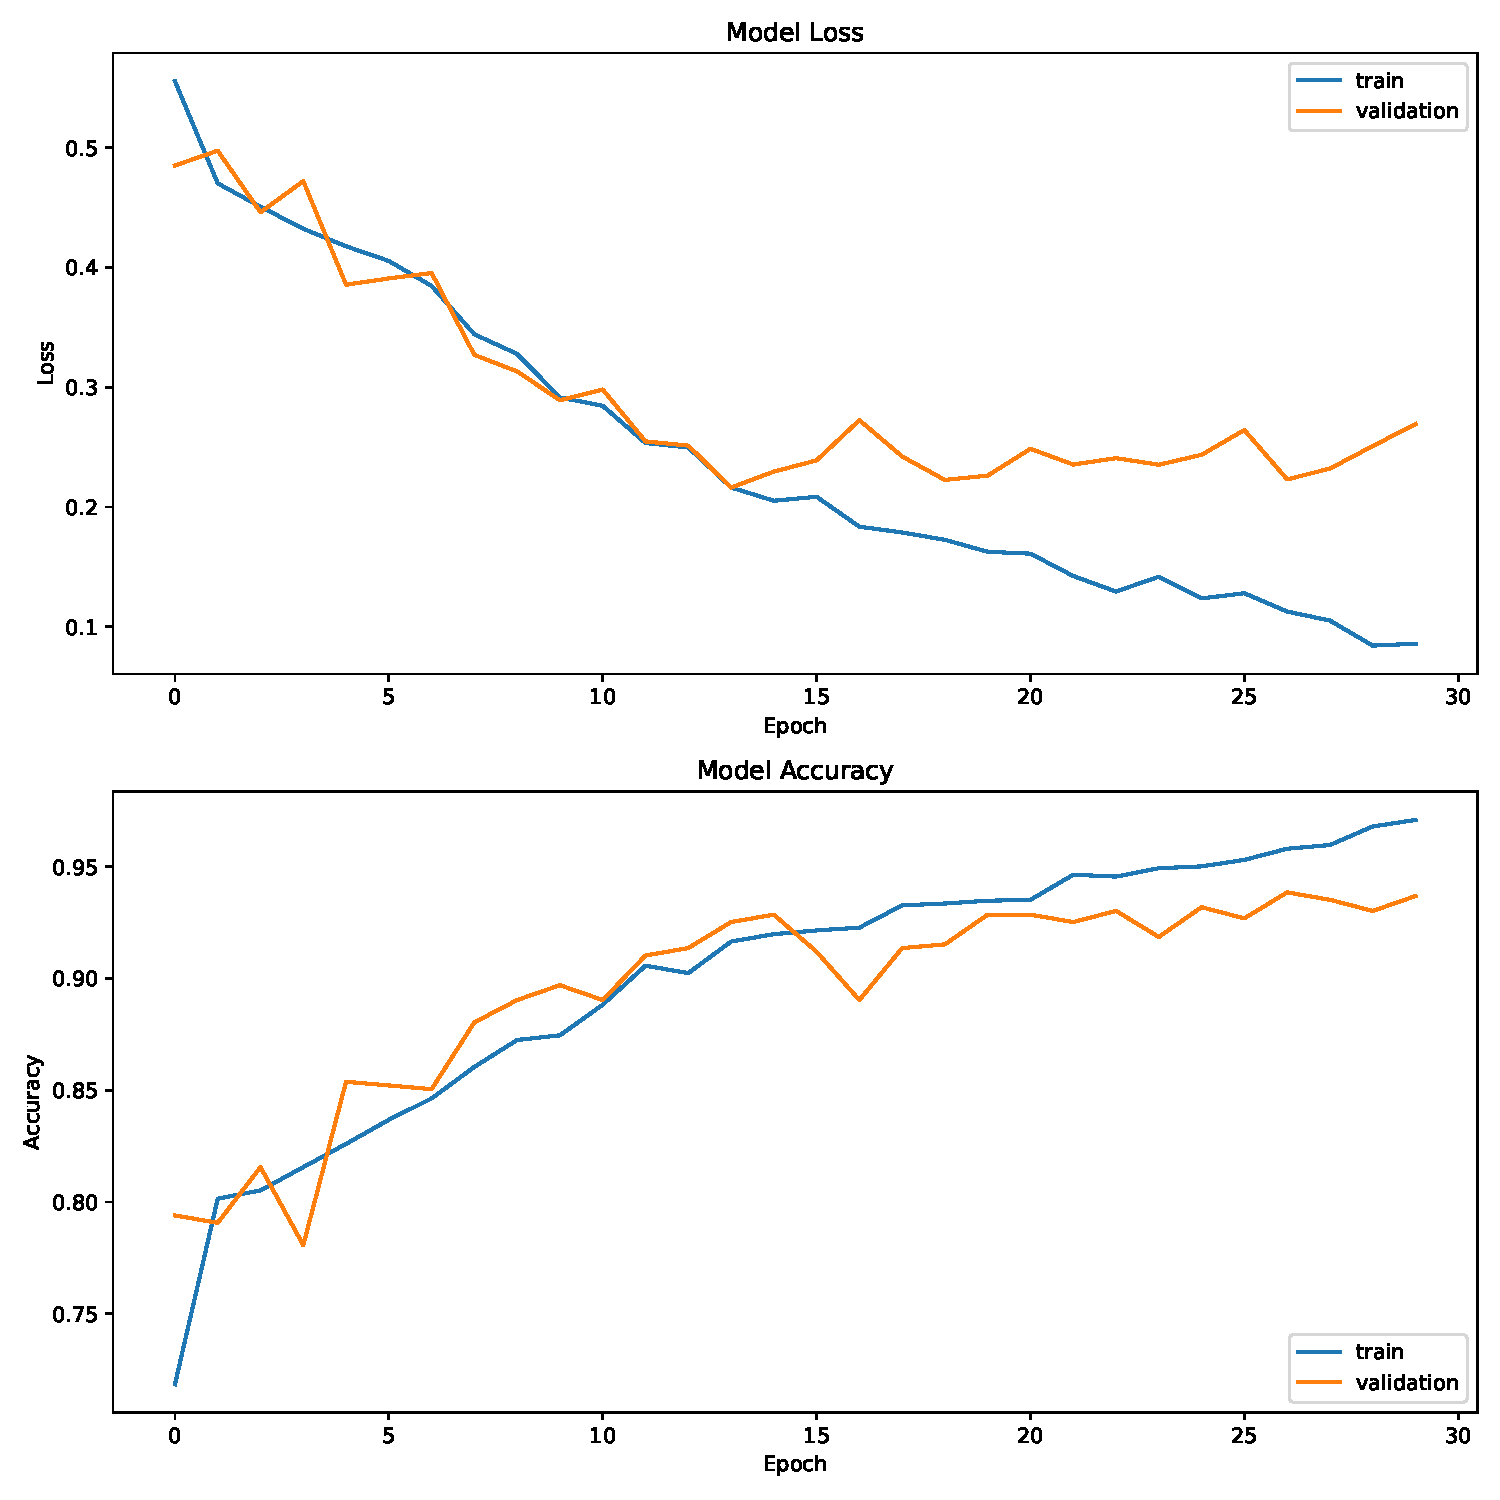
\includegraphics[width=.65\textwidth]{plots/CNN_history.pdf}
    \caption{Accuracy- and loss-curves for the initial CNN.}
    \label{fig:learningCurveInitial}
\end{figure}
\begin{wrapfigure}{r}{5cm}
    \centering
    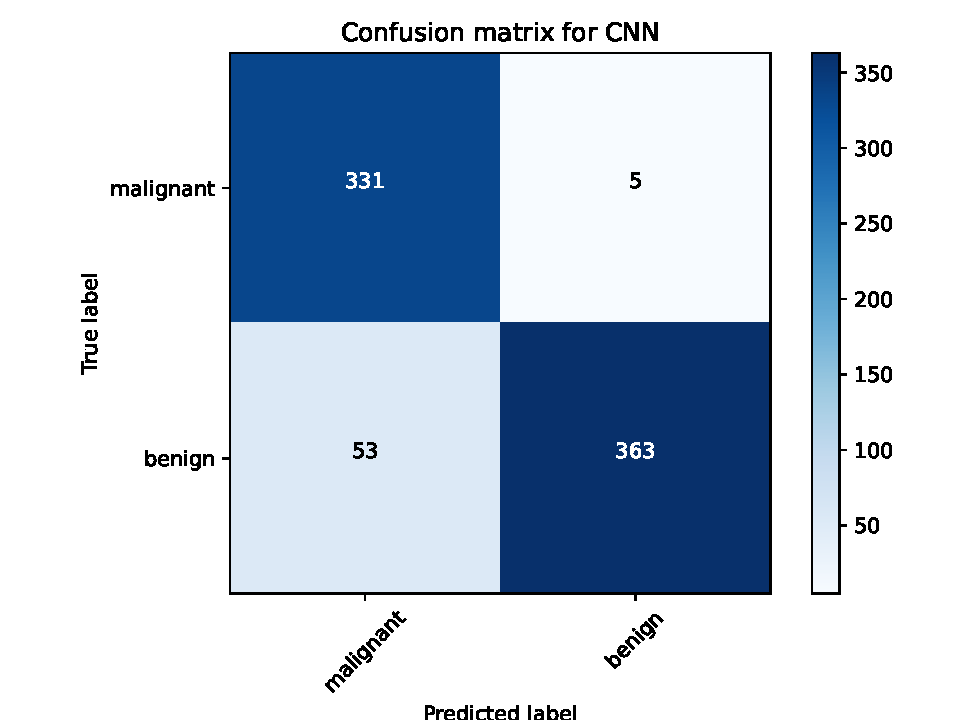
\includegraphics[width=.48\textwidth]{plots/confusion_matrix_CNN.pdf}
    \caption{Confusion matrix for the initial CNN.}
    \label{fig:confusionMatrixInitial}
    \rule{4cm}{0cm}
\end{wrapfigure}
As the model showed high overfitting, which was indicated by the large difference between the training and validation accuracy, a dropout layer with a dropout rate of 0.5 was added to the model.
The learning rate of the Adam optimizer was also increased from $0.001$ to $0.005$ to counteract the overfitting.
The model was retrained for 30 epochs and the accuracy- and loss-curves are shown in figure \ref{fig:learningCurveInitial}.
The learning curves show a high accuracy already, but the model is still overfitting as can be seen by the diverging training and validation loss beginning at around the 13th epoch.
\newline
To further investigate the model, a confusion matrix was created, which is shown in figure \ref{fig:confusionMatrixInitial}.
The confusion matrix shows that the model has a high accuracy for the benign tumours, but a low accuracy for the malignant tumours.
It classifies more benign tumours as malignant than the other way around, which is the desired behaviour.
The metrics for the initial model are shown in the summary below.
\begin{align}
    \label{eq:metricsInitialCNN}
    \begin{split}
        \text{recall} &= 0.8726, \\
        \text{accuracy} &= 0.9229, \\
        \text{precision} &= 0.9864, \\
        \text{f1-score} &= 0.9260, \\
        R^2\text{-score} &= 0.6880, \\
        \text{Mean Squared Error} &= 0.0771.
    \end{split}
\end{align}
It can be seen that the precision and the accuracy are both very high even though an accuracy of 92.29\% is not sufficient for a medical application in such a critical field.
More importantly, the recall value of 87.26\% is not high enough as 58 tumours are wrongly classified, which is a lot in a test dataset of only 752 samples.
How good the model is at predicting the actual values is indicated by the $R^2$-score, which is 0.6880, which means it is off by 31.2\%.
These metrics can be improved by running the model for more epochs.
The problem of the high overfitting, however, needs to be resolved first.

\section{Hyperparameter Optimization}
\label{sec:hyperparameter}

To be able to know which of the hyperparameters lead to overfitting, a grid search over a parameter space was performed by iterating over the number of filters in the convolutional layers, the dropout rate, and the number of dense layers.
The network architecture was kept the same as in the initial model, but the hyperparameters were varied.
A preceding grid search was performed before the following one which led to the range of hyperparameters tested.
The preceding grid search is shown in section \ref{sec:FirstGridsearchHyperparameterTests}.
The number of filters in the first convolutional layer was $n_{\text{filters}}$ with $n_{\text{filters}} \in [24, 36, 48, 60, 72]$ with the second and third convolutional layers with $n_{\text{filters}}/2$ and $n_{\text{filters}}/3$, respectively.
Varied other parameters were the dropout rate $do$ with $do \in [0.4, 0.5, 0.6]$ and the number of dense units $n_{\text{dense}}$ with $n_{\text{dense}} \in [4, 8, 12, 16, 20, 24]$.
The last layer was always a dense layer with 2 neurons.
The models were trained for 30 epochs.
Other hyperparameters were kept the same as in the initial model.
The results of the grid search are shown in figure \ref{fig:gridsearch}.
It shows the effect of the individual hyperparameters on the best validation accuracy, the best training accuracy and the difference between the delta accuracy.
The delta accuracy is calculated by subtracting the validation accuracy from the training accuracy and normalizing it by the validation accuracy.
\begin{figure}[H]
    \centering
    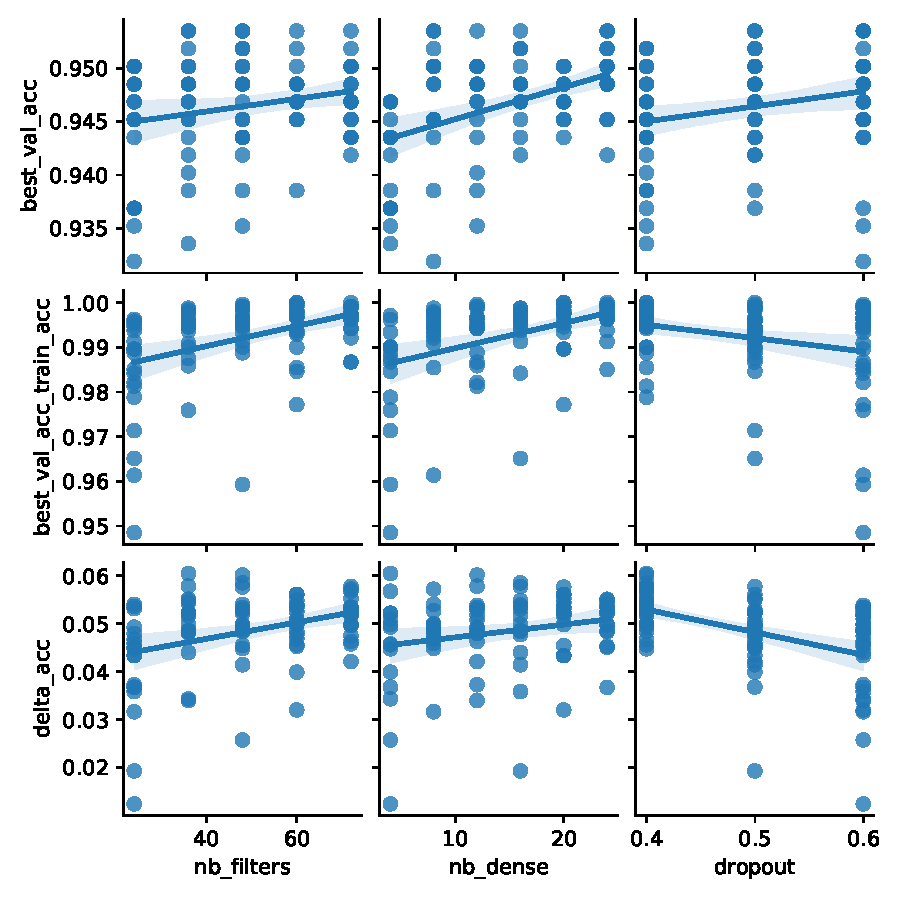
\includegraphics[width=0.65\textwidth]{plots/pairplot.pdf}
    \caption{Hyperparameter testing using a grid search.}
    \label{fig:gridsearch}
\end{figure}
% Figure \ref{fig:gridsearch} shows the effect of the individual hyperparameters on the best validation accuracy, the best training accuracy and the difference between the delta accuracy.

It can be seen that the training and the validation accuracy increase with an increase in the number of filters in the convolutional layers with the effect being more pronounced for the training accuracy.
Increasing the number of filters, however, increases the difference between the training and the validation accuracy, thus leading to more overfitting.
With an increase in dense units, the training and the validation accuracy also increase, with the more pronounced effect being on the validation accuracy.
The delta between the training and the validation accuracy also increases with an increase in dense units, but this effect is less distinctive than with the number of filters.
The dropout rate has a negative effect on the training accuracy and a positive effect on the validation accuracy.
Because of this behaviour, an increase in the dropout rate leads to a decrease in the delta accuracy, thus reducing overfitting.
The first grid search showed similar results, which is why in this grid search the range of dropout rates was increased to a maximum of 0.6 and the range of dense units was increased to a maximum of 24.
The number of filters was not increased, with the only difference being that more filters were tested. %\newline

Figure \ref{fig:gridsearchLearningCurves} shows the learning curves of the best three performing models with figure \ref{fig:SmallestDelta_LearningCurves} showing the models with the least difference in training and validation accuracy and figure \ref{fig:HighestAccuracyLearningCurves} showing the models with the highest accuracy.
\begin{figure}[H]
    \centering
    \begin{subfigure}[B]{.45\textwidth}   % 1st subfigure
        \centering
        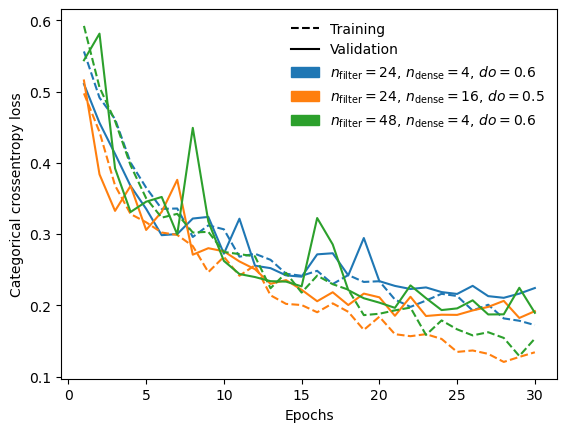
\includegraphics[width=\linewidth]{plots/SmallestDelta_LearningCurves.png}
        \caption{Learning curves of the models with the least difference in training and validation.}
        \label{fig:SmallestDelta_LearningCurves}
    \end{subfigure}    
    \begin{subfigure}[B]{.45\textwidth}   % 2nd subfigure
        \centering
        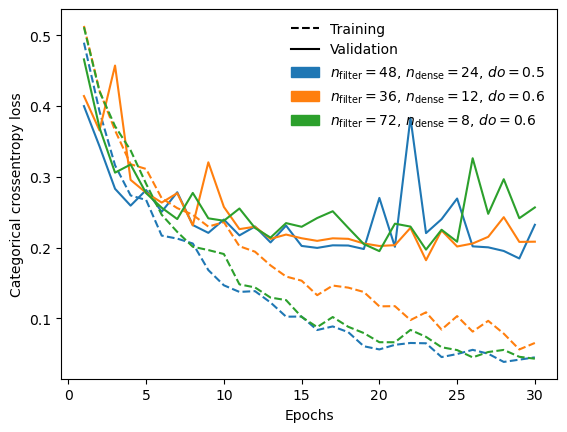
\includegraphics[width=\linewidth]{plots/Best3LearningCurves.png}
        \caption{Learning curves of the models with the highest accuracy.}
        \label{fig:HighestAccuracyLearningCurves}
    \end{subfigure}
    \caption{Learning curves of the models from the grid search.}
    \label{fig:gridsearchLearningCurves}
\end{figure}
What can be seen in figure \ref{fig:SmallestDelta_LearningCurves} is that the models with the least difference in delta accuracy seem like they are not trained enough.
The categorical cross-entropy loss is still decreasing, which means that the models could be trained for more epochs.
That the training and validation loss curves are so close to each other is a promising sign, as it means that the model is not overfitting and that there is still potential for improvement.
The model with the least amount of delta accuracy is also the least complex model with only 24 convolutional filters and 4 dense units.
The dropout rate is 0.6, which is the highest dropout rate tested. \newline
The models with the highest accuracy, however, are already showing signs of overfitting, as can be seen in figure \ref{fig:HighestAccuracyLearningCurves}.
At around the same epoch as in the initial model, the training and validation loss curves start to diverge.
This means that the models are already overfitting and that they should not be trained for more epochs.
The reason for the large overfitting is due to the models being too complex for the amount of data available with the model with the highest accuracy having 48 convolutional filters and 24 dense units and only a dropout rate of 0.5.
The learning curves of the best three performing models in their respective categories in figure \ref{fig:gridsearchLearningCurves} confirm the results from the grid search in figure \ref{fig:gridsearch}.
The model with the least amount of delta accuracy is the one that is chosen for the final model as it shows the least amount of overfitting and still has potential for improvement.

\section{Final Model}
\label{sec:finalModel}

The final model is the model with the least amount of delta accuracy from the grid search.
It is trained for 100 epochs. % with the Adam optimizer and a learning rate of 0.005.
The learning curves for the final CNN are shown in figure \ref{fig:learningCurveFinal}.
\begin{figure}[H]
    \centering
    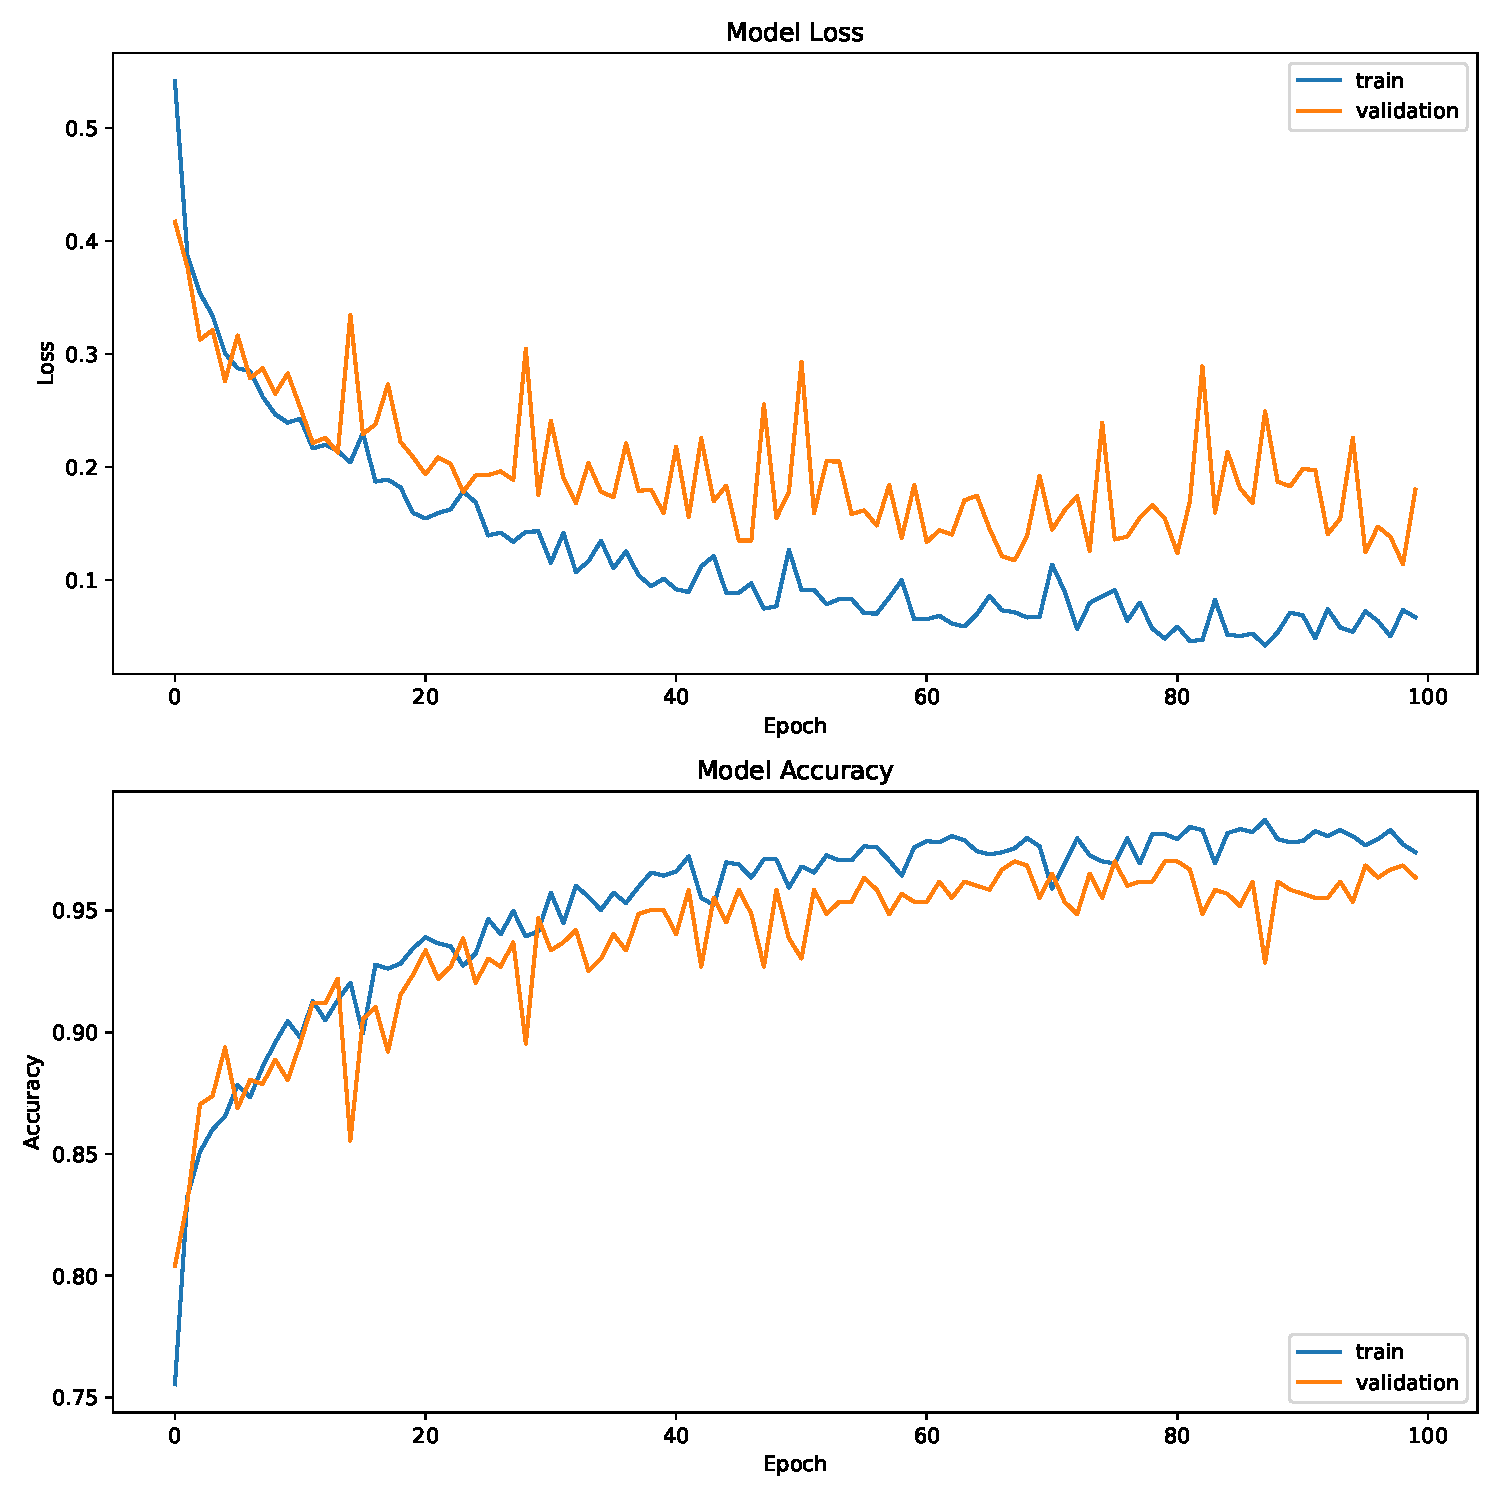
\includegraphics[width=.65\textwidth]{plots/history.pdf}
    \caption{Accuracy- and loss-curves for the final CNN after the hyperparameter optimization.}
    \label{fig:learningCurveFinal}
\end{figure}
The loss curves show that the model does not overfit as much as the initial model, even after 100 epochs, but it also shows that there is still a difference between the training and the validation loss.
As the difference stays constant, the model is not overfitting more with more epochs. 
This difference, however, is lower than in the initial model, indicating that the hyperparameter optimization was successful.
It can also be seen that the validation loss curve has some peaks, which can be explained by the low amount of data available, as the validation loss is calculated on a smaller dataset of 602 samples.
Similar behaviour can be seen in the accuracy curves, with the validation accuracy being lower than the training accuracy.
The difference between the training and the validation accuracy is also smaller than in the initial model.

The confusion matrix for the final model is shown in figure \ref{fig:confusionMatrixFinal}.
It shows similar behaviour as in the final model, with the model classifying more benign tumours as malignant than the other way around.
The amount of tumours that are misclassified, however, is lower than in the initial model.
The metrics for the final model are shown in the summary below.
\begin{wrapfigure}{r}{5cm}
    \centering
    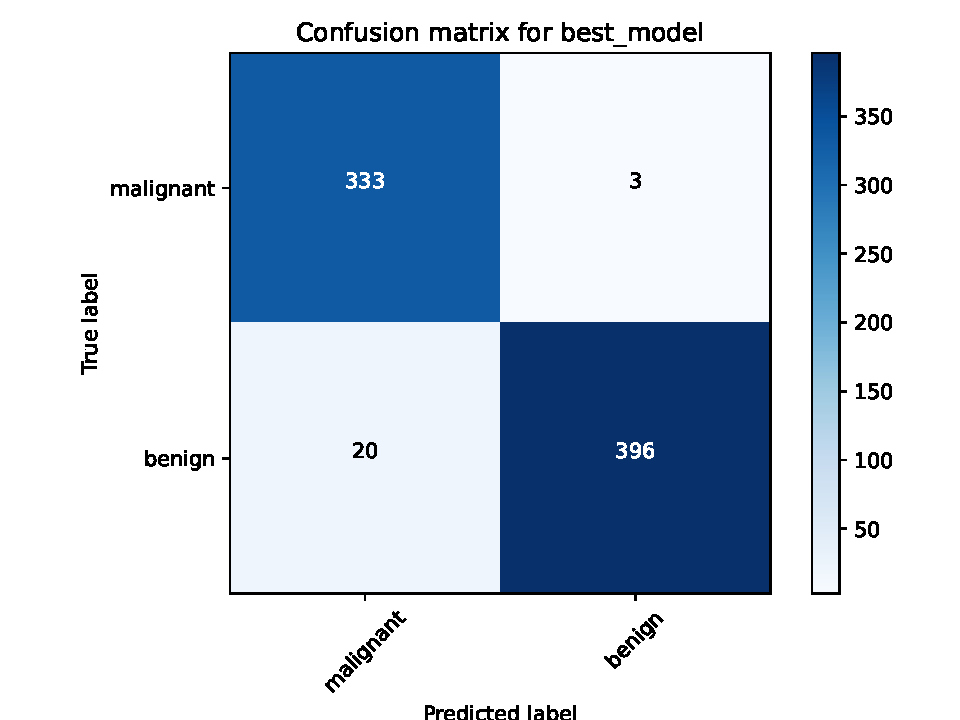
\includegraphics[width=.48\textwidth]{plots/confusion_matrix_best_model.pdf}
    \caption{Confusion matrix for the final CNN after the hyperparameter optimization.}
    \label{fig:confusionMatrixFinal}
\end{wrapfigure}
\noindent
It can be seen that all of the metrics have improved compared to the initial model.
The biggest reason for this improvement is the increase in runtime from 30 to 100 epochs.
But as the initial model was already overfitting at 30 epochs, it made sense to first optimize the hyperparameters as the initial model could just adjust the weights to the training data therefore remembering the training data.
As the final model has shown a significant improvement in the overfitting, the results are more reliable than in the initial model. \newline
\begin{align}
    \label{eq:metricsFinalCNN}
    \begin{split}
        \text{recall} &= 0.9519, \\
        \text{accuracy} &= 0.9694, \\
        \text{precision} &= 0.9925, \\
        \text{f1-score} &= 0.9718, \\
        R^2\text{-score} &= 0.8763, \\
        \text{Mean Squared Error} &= 0.0306.
    \end{split}
\end{align}
% The recall value of 95.19\% is much better than in the initial model. 
% The improvement in the recall value is the most important as it is the metric that is most important for a medical application.
% The accuracy has improved to 96.94\%.
As said before, the recall value is the most important metric for a medical application.
The recall value of 95.19\% is much better than in the initial model.
The accuracy has improved to 96.94\%. 
The precision value of 99.25\% is very high and the F1-score of 97.18\% is also very good.
The $R^2$-score of 87.63\% is also a good value, as it means that the model is off by 12.37\%. \newline
As all of the metrics have improved while the model is not overfitting as much as in the initial model, the final model is a significant improvement over the initial model.

\chapter{Alternative Methods}
\label{cha:alternative_methods}



\section{Comparison to the CNN}
\label{sec:comparison}

\begin{table}[H]
    \centering
    \caption{Comparison of the alternative methods to the initial and the final CNN.}
    \label{tab:comparisonTable}
    \begin{tabular}{c | c c c c c c c}
        \toprule
        model & recall & accuracy & precision & f1-score & $R^2$-score & Mean Squared Error \\%& Mean Absolute Error \\
        \midrule
        SVM & 0.9617 & 0.9801 & 0.9939 & 0.9775 & 0.9195 & 0.0199 \\
        LR & 0.9617 & 0.9788 & 0.9909 & 0.9760 & 0.9141 & 0.02124 \\
        kNN & 0.9469 & 0.9761 & 1.0 & 0.97273 & 0.9034 & 0.0239 \\
        CNN & 0.8726 & 0.9229 & 0.9864 & 0.926 & 0.688 & 0.0771 \\
        best model & 0.9519 & 0.9694 & 0.9925 & 0.9718 & 0.8763 \\ 
        \bottomrule
    \end{tabular}
\end{table}
\chapter{Conclusion}
\label{cha:conclusion}


$\vdots$



\appendix
% Hier beginnt der Anhang, nummeriert in lateinischen Buchstaben
\chapter{Appendix}
\label{cha:appendix}

\section{Data Exploration}
\label{sec:DataExploration}

% \begin{figure}[H]
%     \centering
%     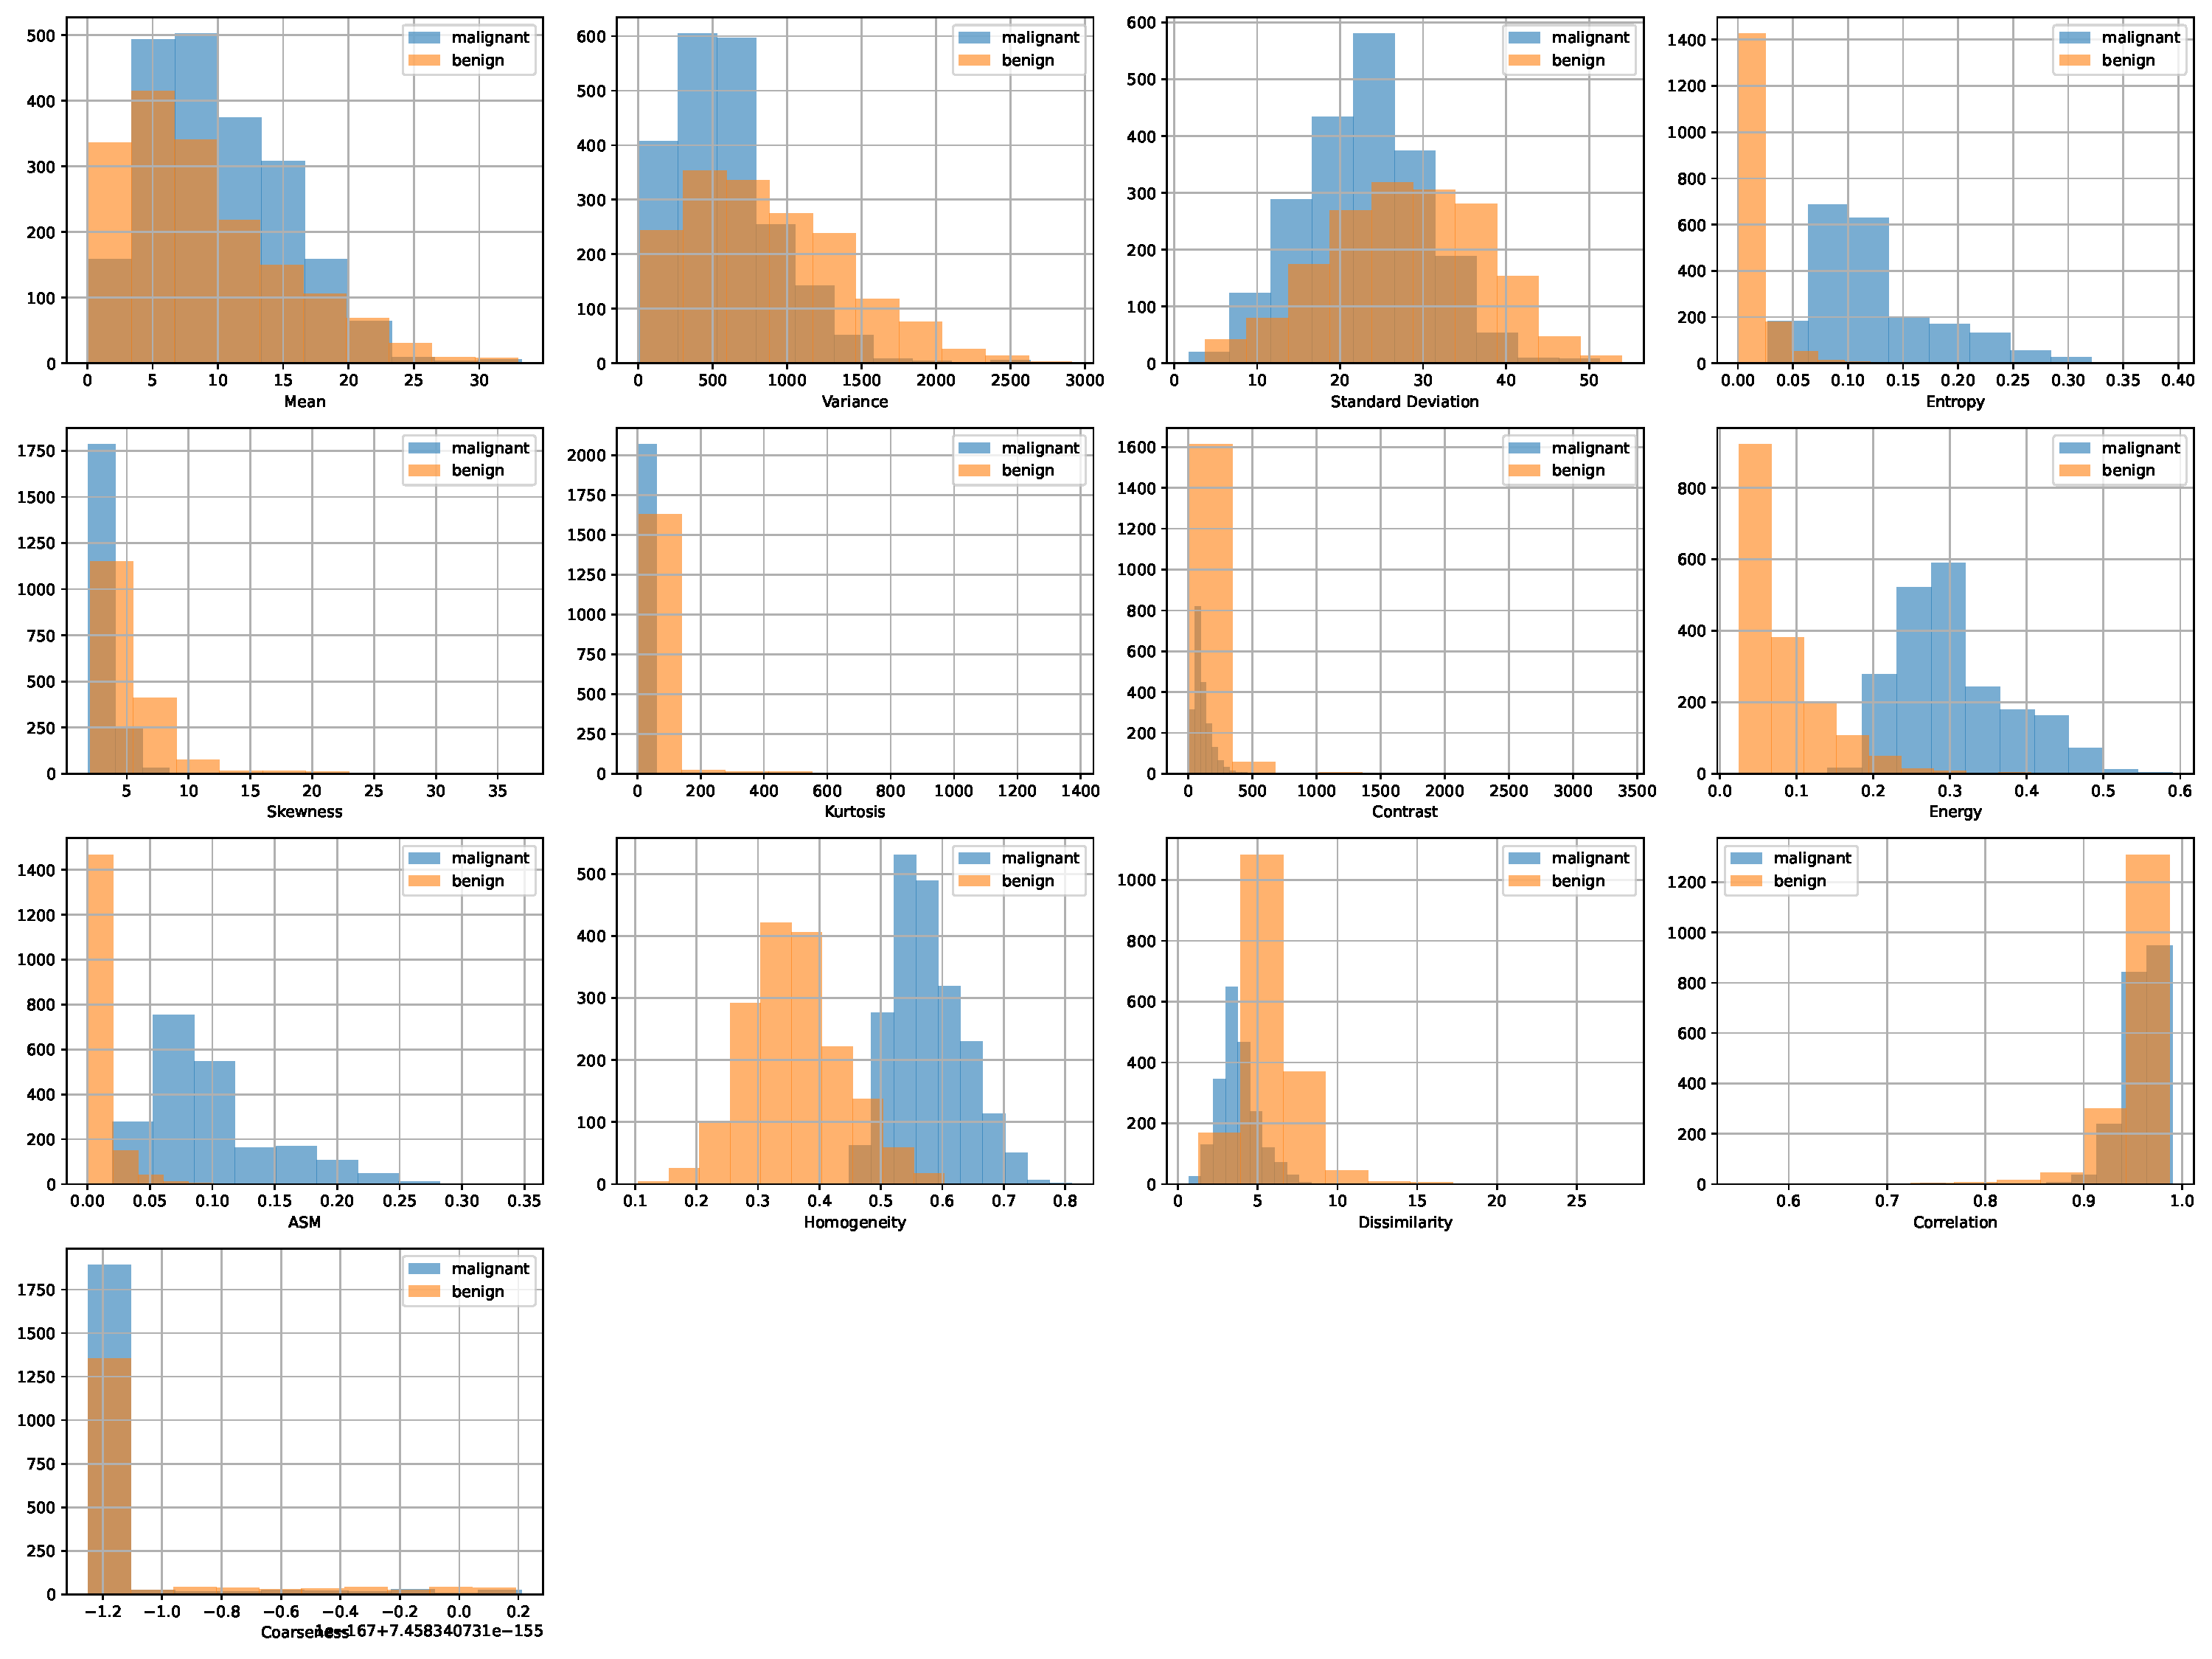
\includegraphics[width=.8\textwidth]{plots/benign_malignant_comparison.pdf}
%     \caption{Comparison between benign and malignant brain tumours for the first- and second-order features.}
%     \label{fig:benign_malignant_comparison}
% \end{figure}

The correlation and scatter matrix of the first- and second-order features are shown in figures \ref{fig:correlation} and \ref{fig:scatter_matrix} respectively.

\begin{figure}[H]
    \centering
    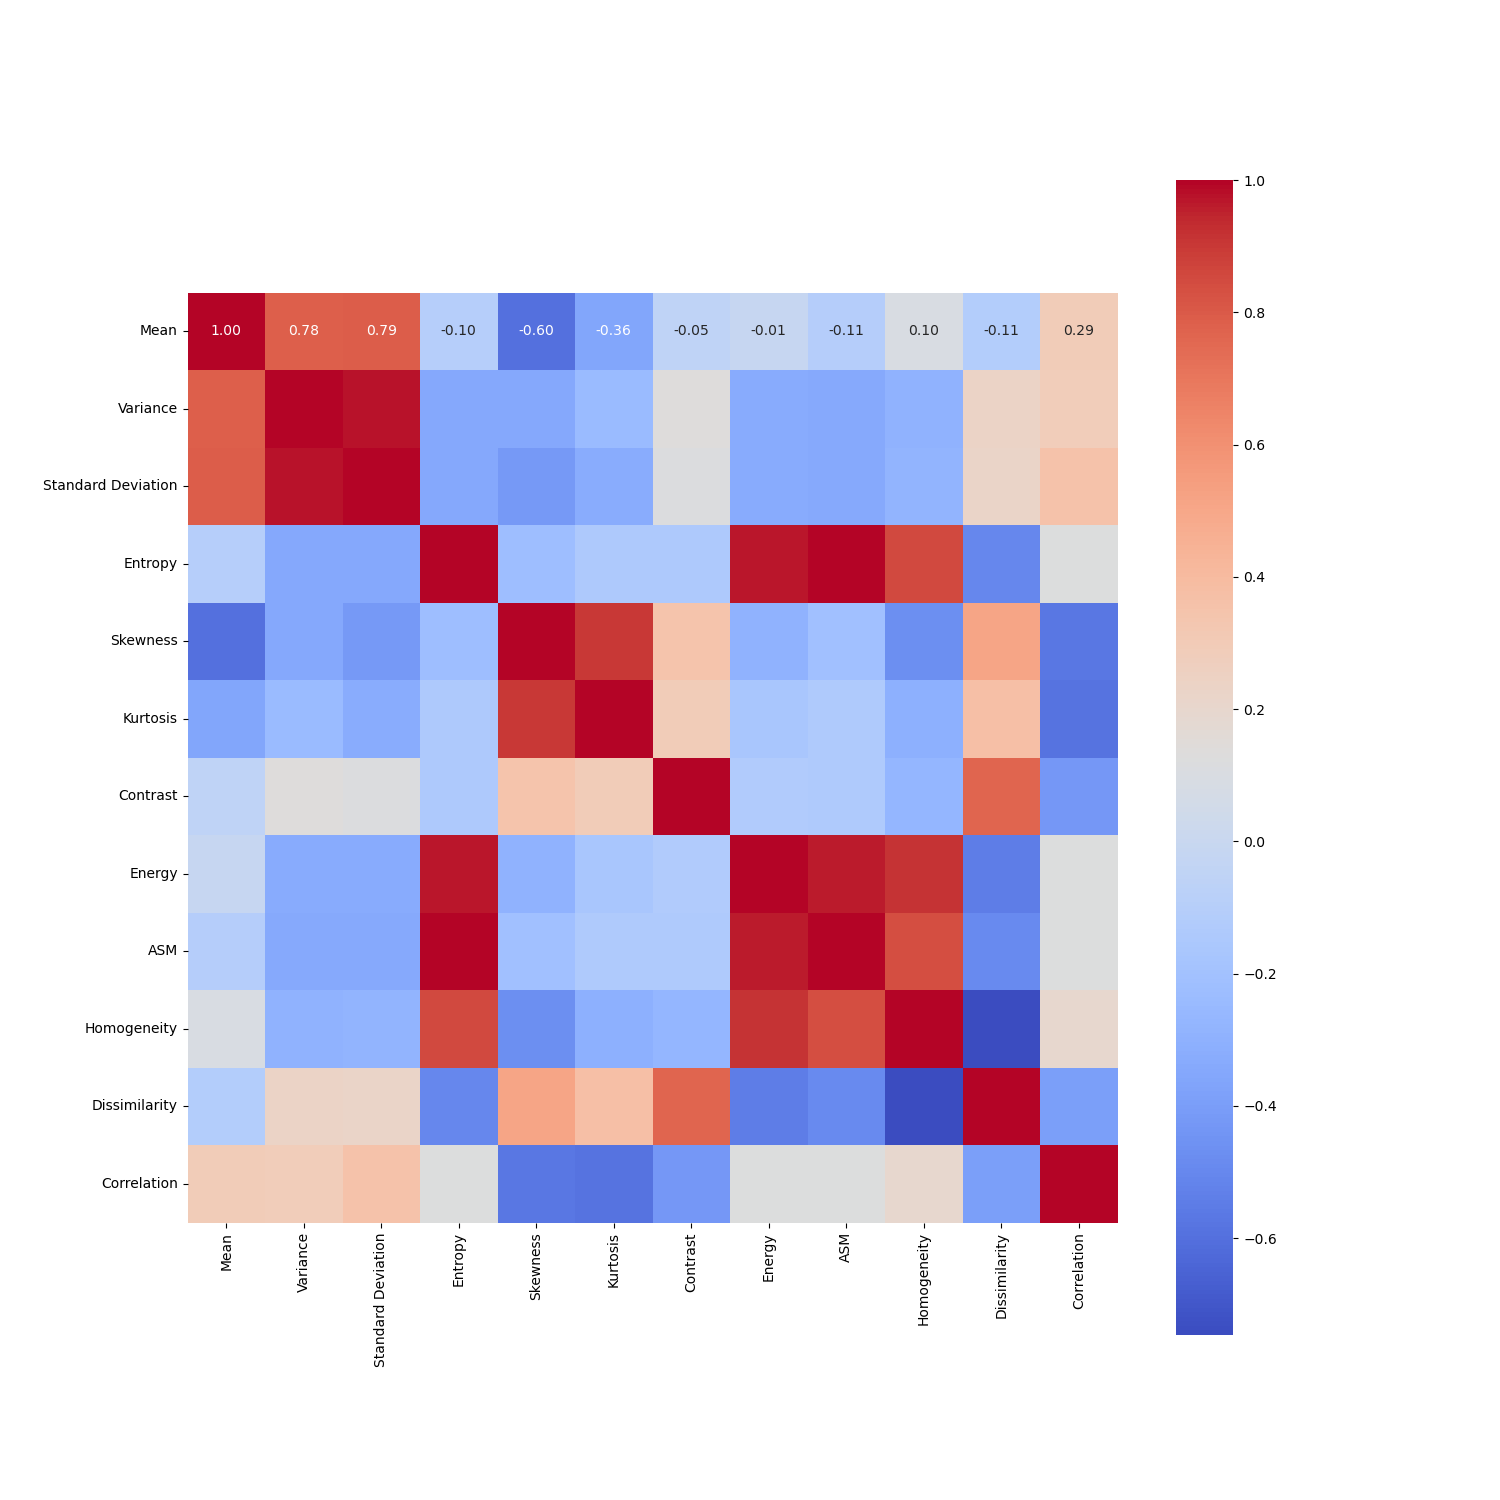
\includegraphics[width=.8\textwidth]{plots/correlation.png}
    \caption{Correlation of the first- and second-order features.}
    \label{fig:correlation}
\end{figure}

\begin{figure}[H]
    \centering
    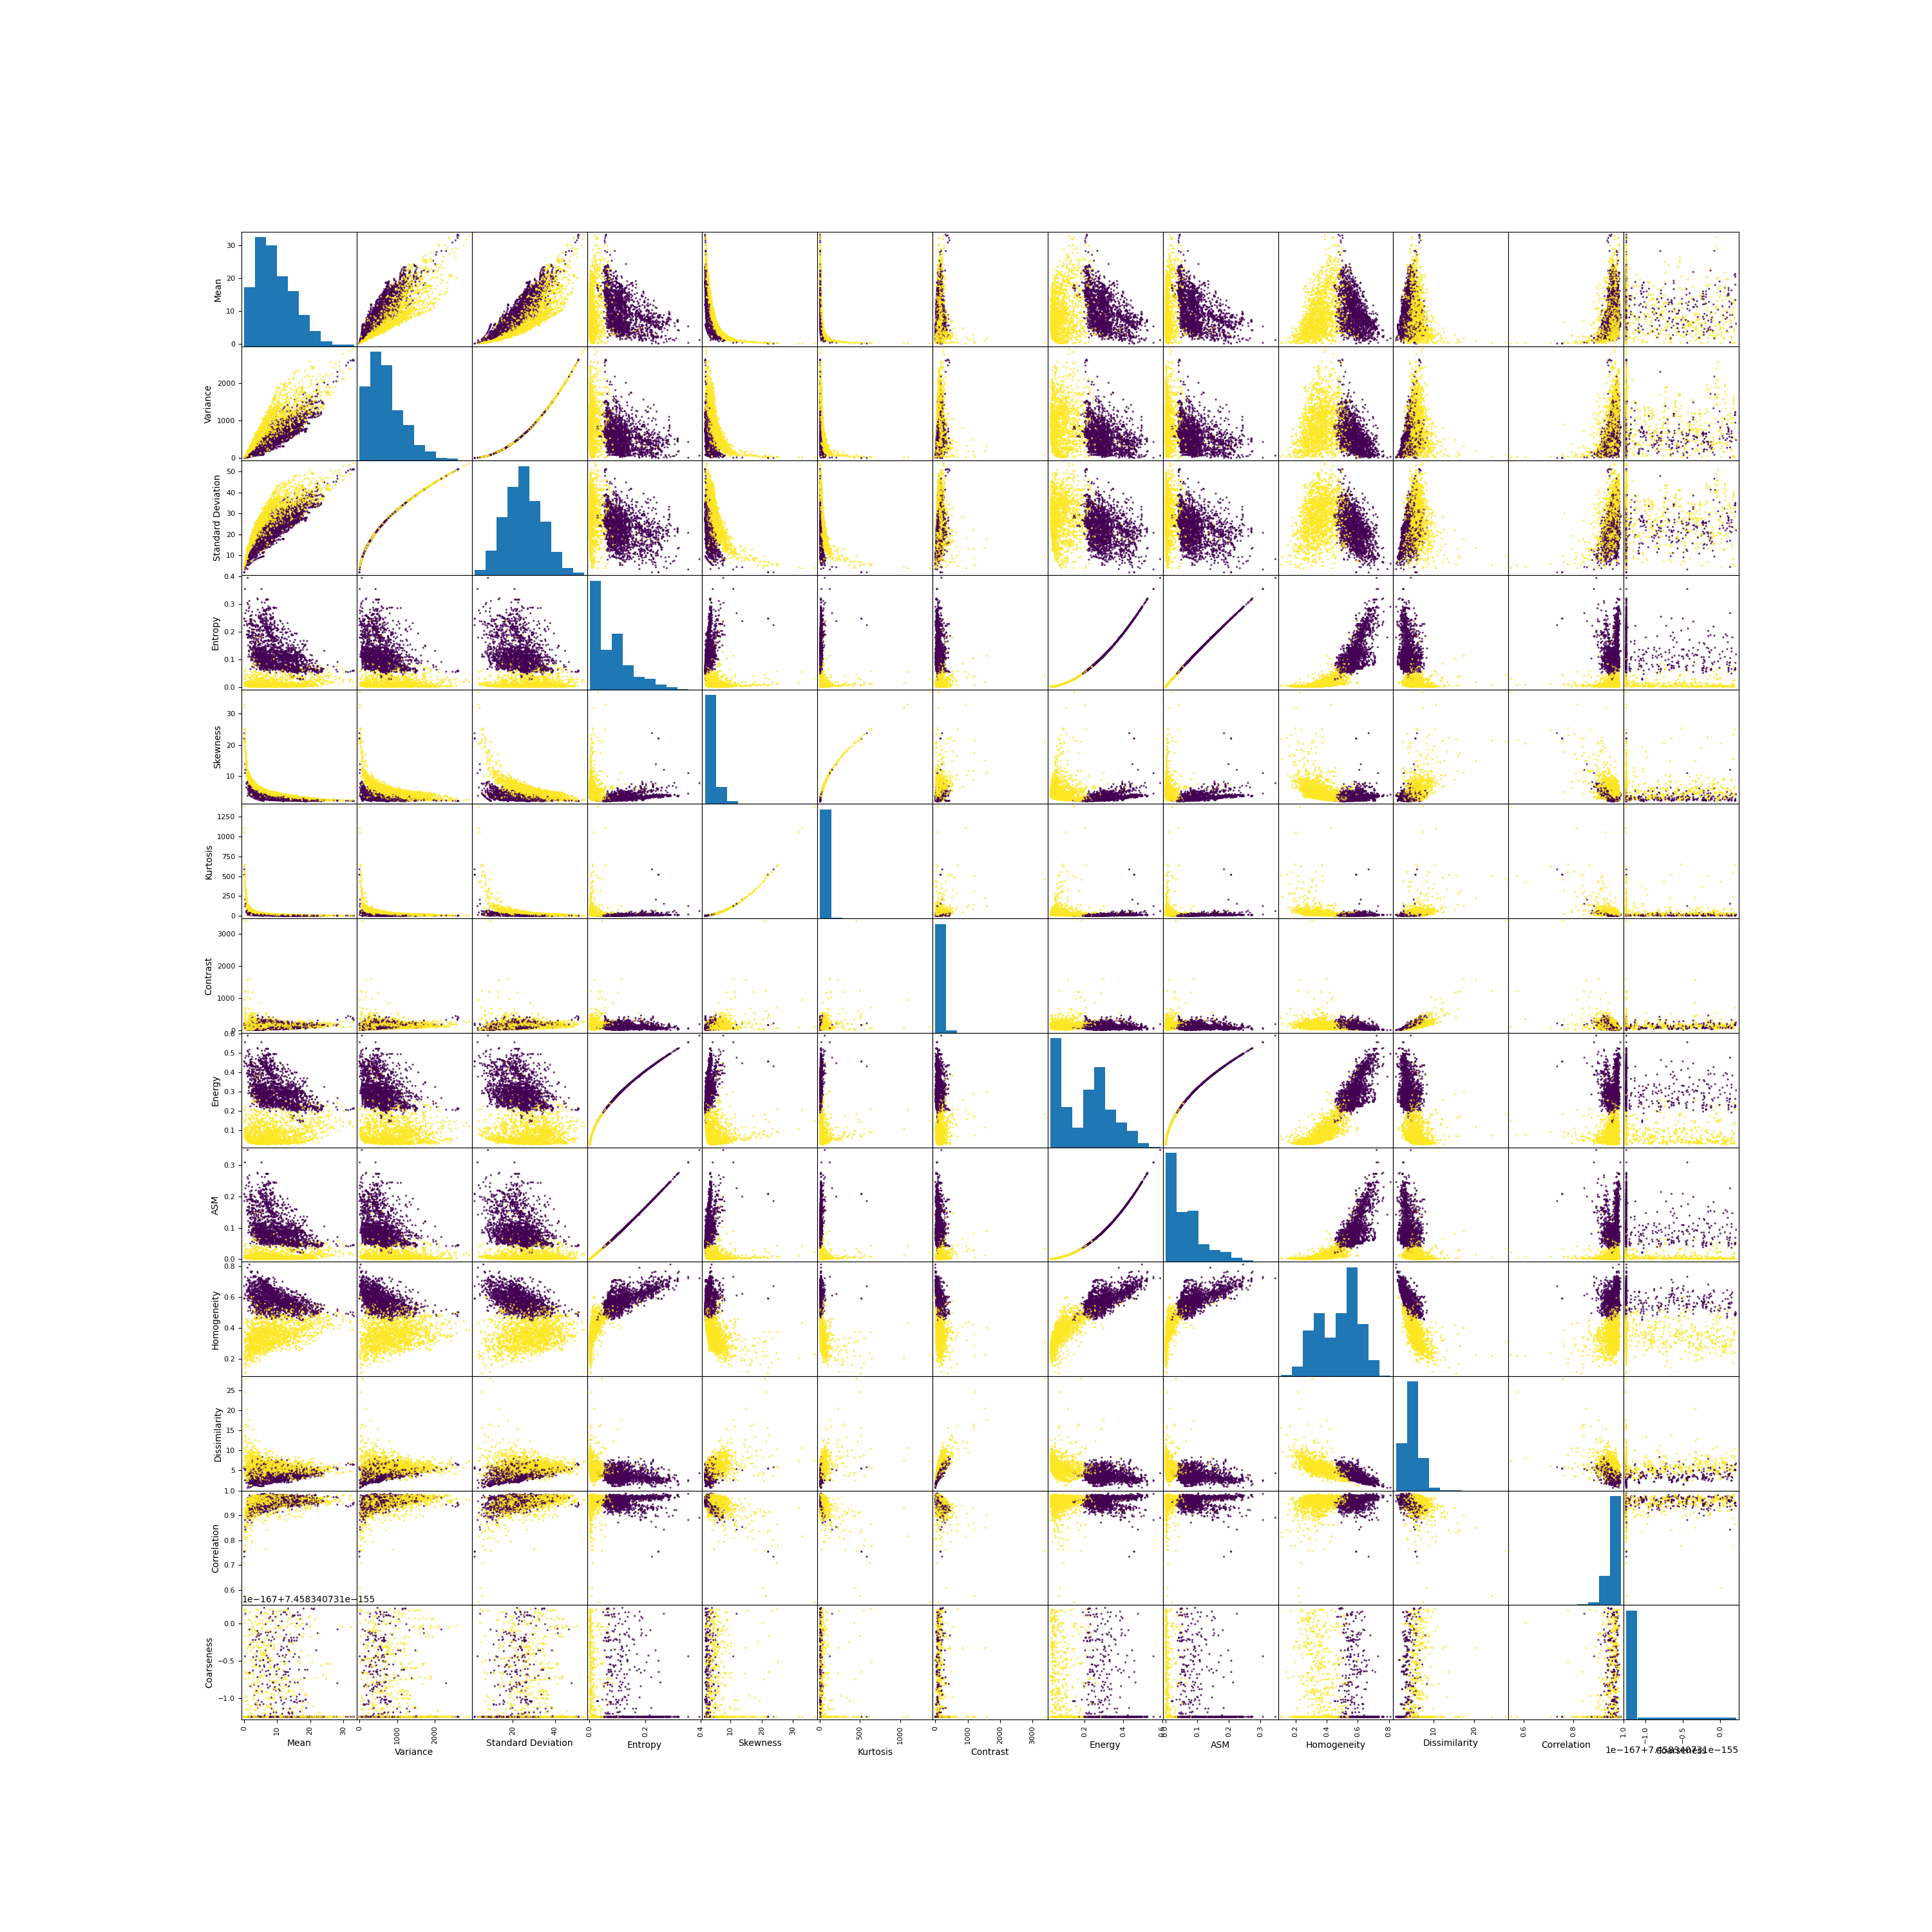
\includegraphics[width=.8\textwidth]{plots/scatter_matrix.png}
    \caption{Scatter matrix of the first- and second-order features.}
    \label{fig:scatter_matrix}
\end{figure}


\section{First Gridsearch Hyperparameter Tests}
\label{sec:FirstGridsearchHyperparameterTests}

Figure \ref{fig:FirstHyperparameterTests} shows the first hyperparameter tests using gridsearch.
This hyperparameter test led to the test, which is described in section \ref{sec:hyperparameter}.
The main goal was to reduce the overfitting, which is why the delta between the training and validation loss was used as the main metric. 
Because the dropout rate decreased the delta between the training and validation loss so much, it was decided to increase the dropout range to 0.6 in the next test.
Because the number of dense units did not have an impact on the delta, a higher range was chosen for the next test.
The range of the number of filters in the convolutional layers was not increased as the delta increased with the number of filters.
There was only taken more data for the next test by using more filters in the same range.

\begin{figure}[H]
    \centering
    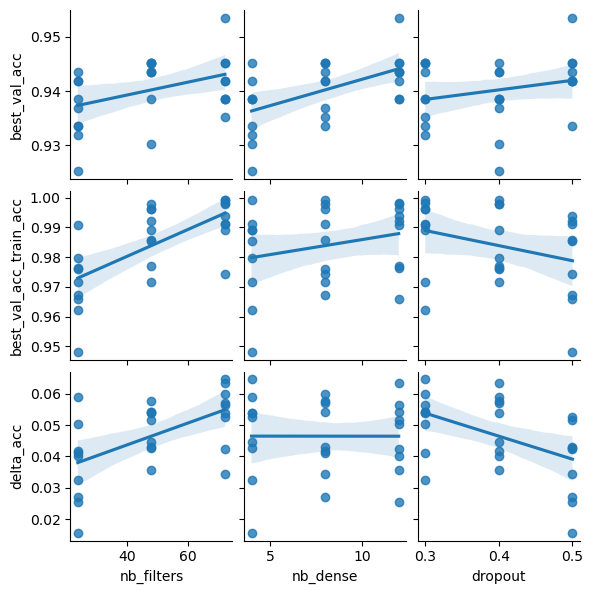
\includegraphics[width=.8\textwidth]{plots/FirstHyperparameterTests.png}
    \caption{First hyperparameter tests using gridsearch.}
    \label{fig:FirstHyperparameterTests}
\end{figure}



\backmatter
\printbibliography

% \cleardoublepage
% From https://www.tu-dortmund.de/studierende/im-studium/pruefungsangelegenheiten/allgemeine-vordrucke/
% 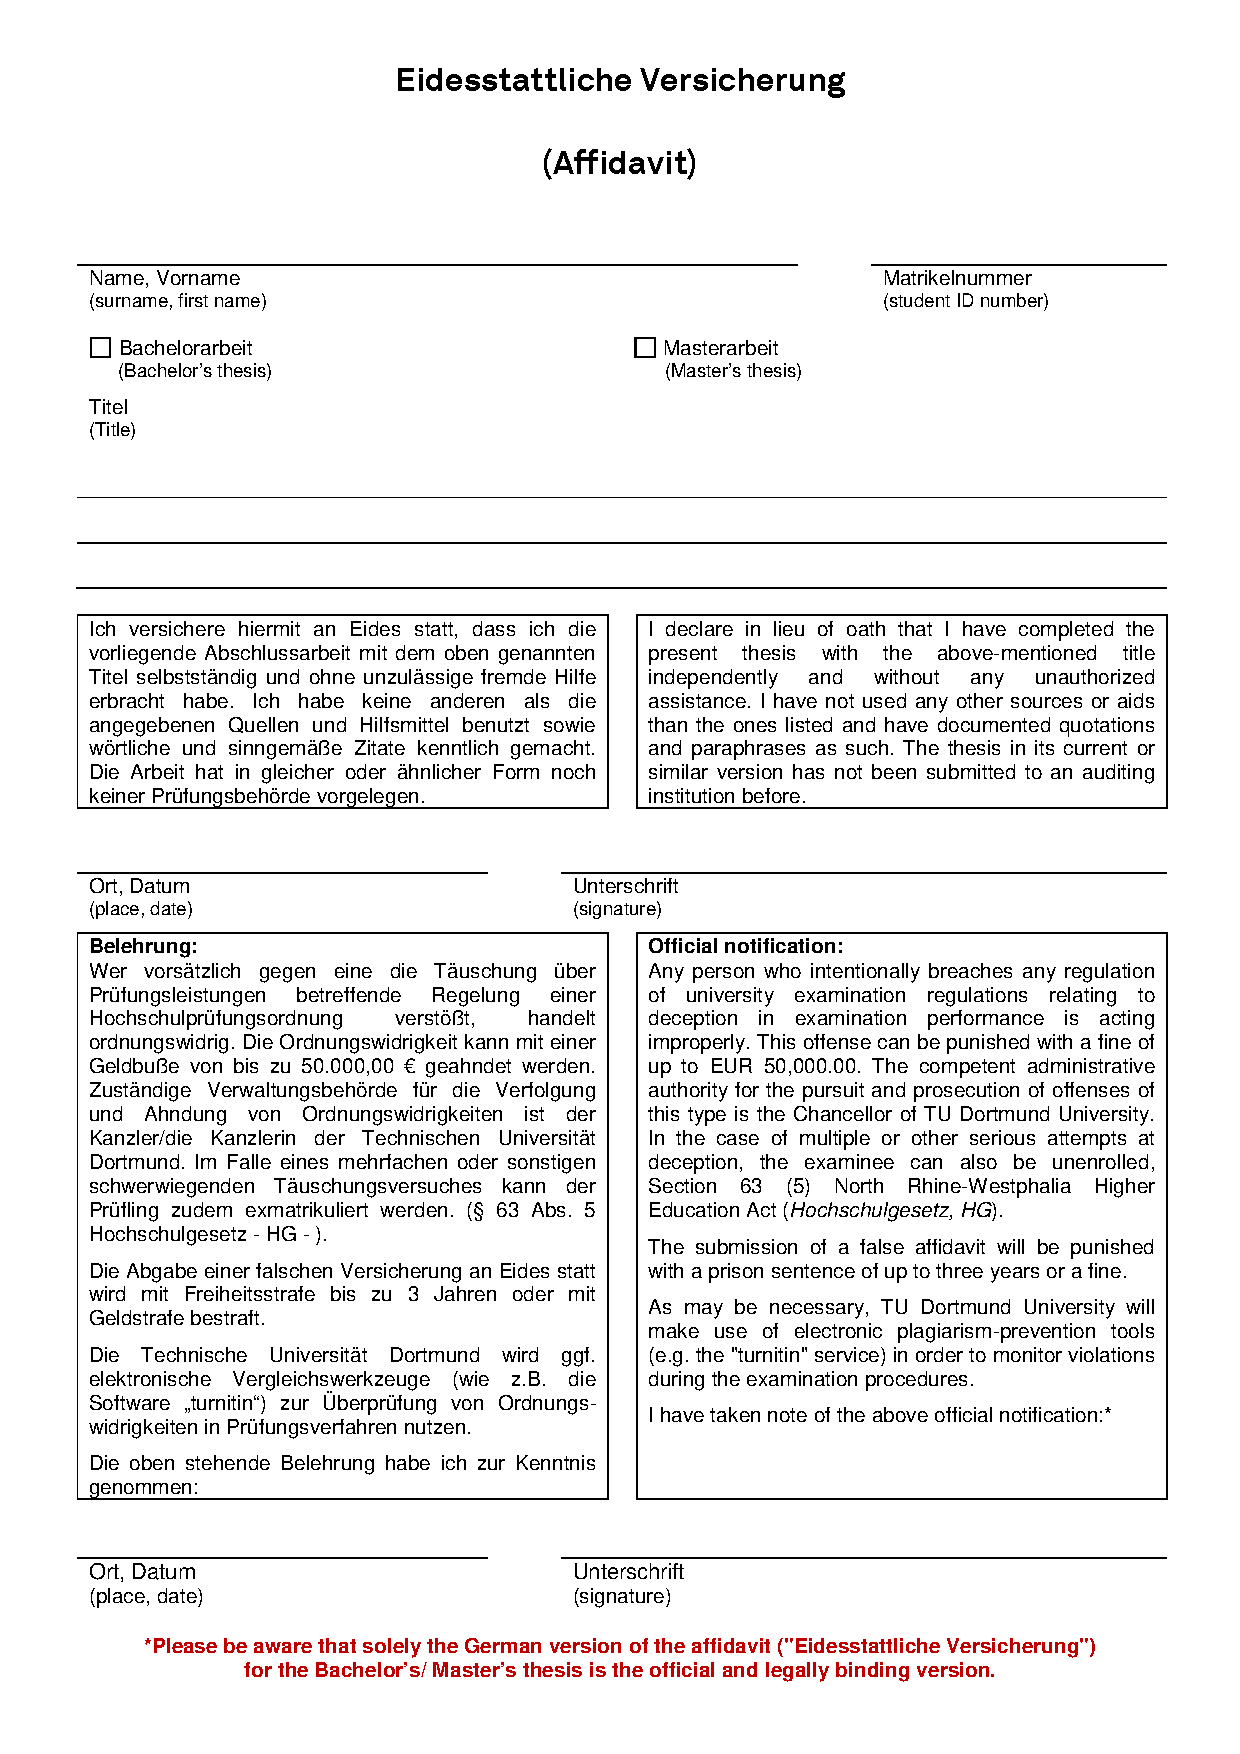
\includepdf{content/Eidesstattliche_Versicherung.pdf}

\end{document}
